\documentclass[10pt, twoside]{report}

\usepackage[T1]{fontenc}
\usepackage[utf8]{inputenc}
%%\usepackage[us]{babel}
\usepackage{helvet}
\usepackage[a4paper,width=180mm,top=25mm,bottom=25mm,bindingoffset=6mm]{geometry}
\usepackage[framemethod=default]{mdframed}
\usepackage{lipsum,titlesec,xcolor,fancyhdr,array,multicol,float,graphicx,wrapfig,subcaption}
\usepackage{fontspec,todonotes,enumitem,comment,capt-of,amsmath,booktabs}
\usepackage[colorlinks]{hyperref}
\usepackage[font=scriptsize]{caption}
\usepackage[sorting=none]{biblatex}
\addbibresource{references.bib}

\DeclareCaptionLabelFormat{andtable}{#1˜#2 \& \tablename˜\thetable}

\renewcommand{\familydefault}{\sfdefault}

\graphicspath{{images/}}

%% define size for chapter initial page:
\usepackage{titlesec, blindtext, color}
\definecolor{gray75}{gray}{0.75}
\newcommand{\hsp}{\hspace{20pt}}
\titleformat{\chapter}[hang]{\Huge\bfseries}{\thechapter\hsp\textcolor{gray75}{|}\hsp}{0pt}{\Huge\bfseries}

\titlespacing*{\chapter}{0pt}{-60pt}{20pt} %% change spacing
%%%%%%%%%%

\floatstyle{plain}
\restylefloat{figure}

\pagestyle{fancy}
\fancyhf{}
\renewcommand{\chaptermark}[1]{ \markboth{#1}{} }
\renewcommand{\sectionmark}[1]{ \markright{#1}{} }
\fancyhead[LE]{\itshape{ \fontsize{10}{12} \selectfont \leftmark}}
\fancyhead[RE, LO]{\thepage}
\fancyhead[RO]{\itshape{\fontsize{10}{12} \selectfont \rightmark}}
\renewcommand\headrulewidth{0pt}

 \hypersetup{
     colorlinks,
     citecolor= green,
     filecolor=black,
     linkcolor= black,
     urlcolor=blue
 }


\begin{document}
    \begin{titlepage}
    \centering
    
\includegraphics[width=0.30\textwidth]{images/cherubino_black.pdf}\par\vspace{1cm}
    {\scshape\LARGE Università di Pisa \par}
    \vspace{1cm}
    {\scshape\ Social Network Analysis \\A.A. 2017/2018\par}
    \vspace{1.5cm}
    {\huge\bfseries Cambridge Analytica and Facebook: \\ The Scandal and the Fallout on Twitter\\ \par}
    \vspace{2cm}
    {\Large Gianmarco Ricciarelli 555396 \\ Stefano Carpita 304902 \par}
    \vfill

\begin{flushright}    
  \textit{Data drives all we do.}\\
\vspace{2 mm}
Cambridge Analytica main slogan.
\end{flushright}

\vspace{4 mm}
    
\begin{flushright}    
  \textit{Rules don’t matter for them. \\ For them, this is a war, and it’s all fair.}\\
\vspace{2 mm}
  Christopher Wylie, \\ former datascientist at Cambridge Analytica, about its leaders.
\end{flushright}




  \end{titlepage}


    \pagenumbering{Roman}
    \tableofcontents
    \chapter{The case story}
    \pagenumbering{arabic}

On Saturday 17 of March 2018, the newspapers The Observer and The New York Times broke reports on how the consulting firm Cambridge Analytica harvested private information from the Facebook profiles of more than 50 million users without their permission, making it one of the largest data leaks in the social network’s history. \cite{nyt_17march}. REF OBSERVER

The whistleblower Christopher Wylie, datascientist and former director of research at Cambridge Analytica revealed...
Cambridge Analytica described itself as a company providing consumer research, targeted advertising and other data-related services to both political and corporate clients.

What, Where, Who, Why, Where ?


Timeline da sistemare: \cite{nyt_timeline}
\begin{itemize}

\item March 17, 2018: The Observer and The New York Times publish joint reports on data harvesting by Cambridge Analytica. UK Information Commissioner Elizabeth Denham issues statement that they are “investigating circumstances in which Facebook data may have been illegally acquired and used.” Politicians in US and UK call for investigation.

\item March 19, 2018: Channel 4 News publishes part 1 of their undercover investigation into Cambridge Analytica. Facebook sends investigators to Cambridge Analytica’s offices. UK Information Commissioner orders them to stand down.

\item March 20, 2018: Channel 4 News publishes part 2 of their undercover investigation into Cambridge Analytica, where they boast about getting Donald Trump elected. British MP Damian Collins calls on Facebook to present oral evidence on Cambridge Analytica. Facebook agrees to send former operations manager Sandy Parakilas. Facebook holds internal Q\&A with attorney Paul Grewal to discuss the crisis, but CEO Mark Zuckerberg and COO Sheryl Sandberg do not attend. Cambridge Analytica suspends CEO Alexander Nix. Facebook demands to inspect Christopher Wylie’s phone. FTC opens investigation into Facebook.
\item to be continued...
\end{itemize}

    \chapter{Building the network}

    \begin{figure}[htbp]
      \centering
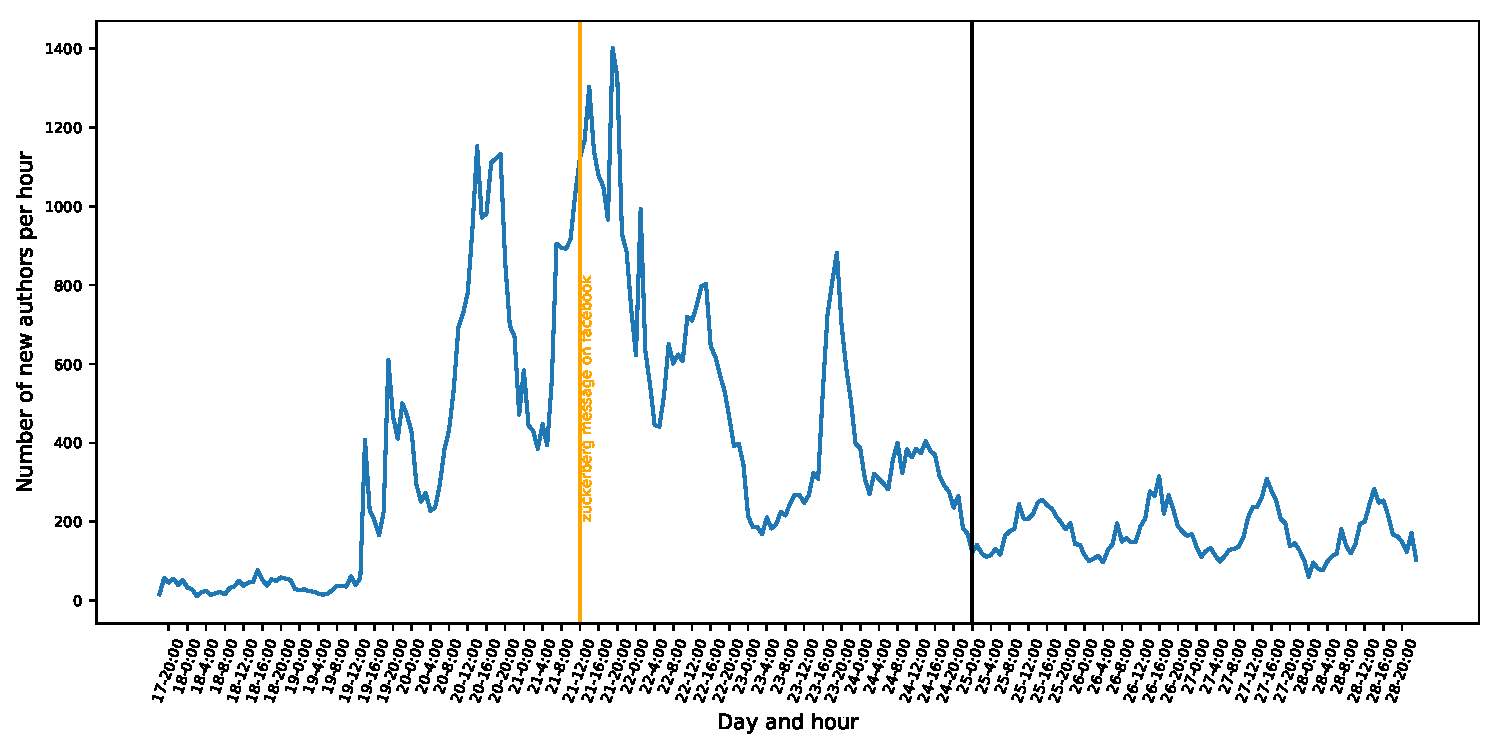
\includegraphics[width=\textwidth]{../../scripts/visualization/imgs/time_history.pdf}            
      \caption{New authors time history}
      \label{fig:time_history}
    \end{figure}

    
    \chapter{Network properties}

    
    \begin{figure}[htbp]
      \centering
      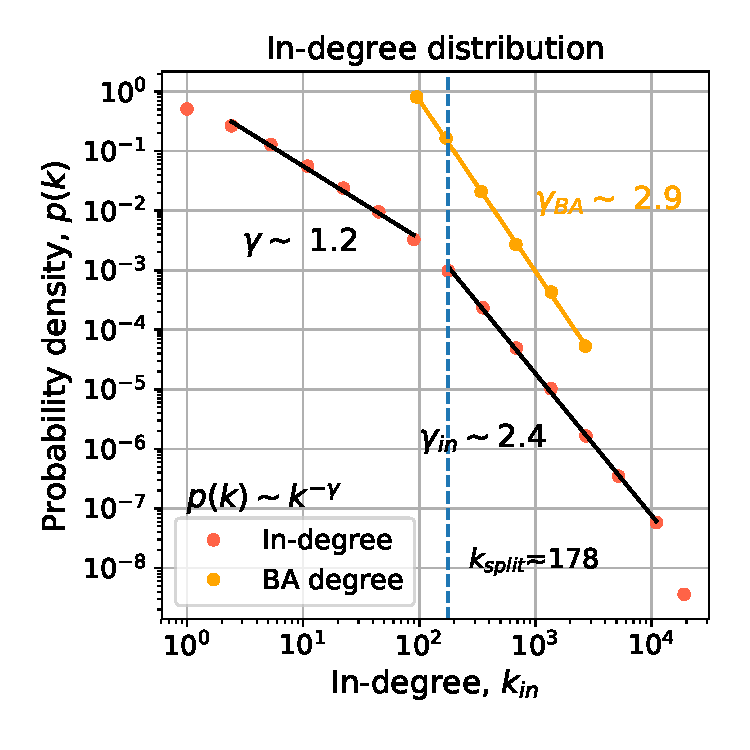
\includegraphics[width=\textwidth]{../../scripts/visualization/imgs/in_degree_distribution.pdf}            
      \caption{New authors time history}
      \label{fig:time_history}
    \end{figure}

    
    \chapter{Network dynamics}

    \chapter{Communities discovery}

    \chapter{Spreading}
    \chapter{Spreading} % (fold)
\label{cha:spreading}

In this chapter we'll describe the results we obtained by applying the \textbf{SI}, \textbf{SIS}, \textbf{SIR},
and \textbf{Threshold} diffusion models both on the crawled data and on the synthetic graphs (Erdős–Rényi and
Barabási–Albert) generated from the original one. In each section, a comparison between the three networks will be
provided along with some details on the implementation of the tests of every model.

\section{SI model} % (fold)
\label{sec:si_model}
    \begin{figure}[H]
        \centering
        \begin{subfigure}{0.45\textwidth}
            \resizebox{\textwidth}{!}{
                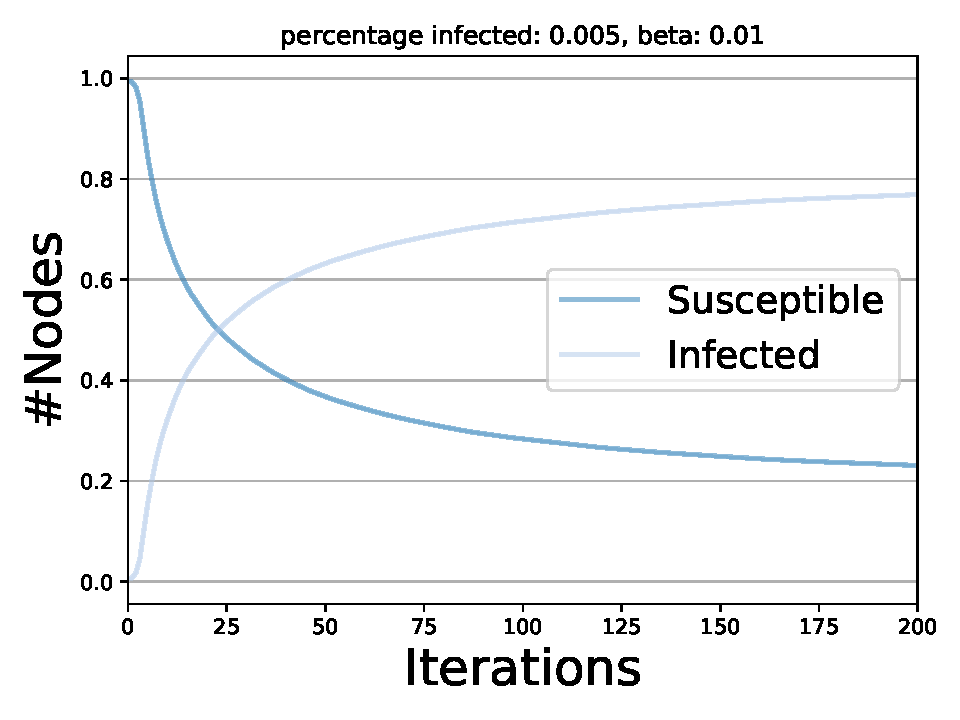
\includegraphics{images/spreading/si/diffusion.pdf}

            }
            \caption{}
            \label{diff_si}
        \end{subfigure}
        \begin{subfigure}{0.45\textwidth}
            \resizebox{\textwidth}{!}{
                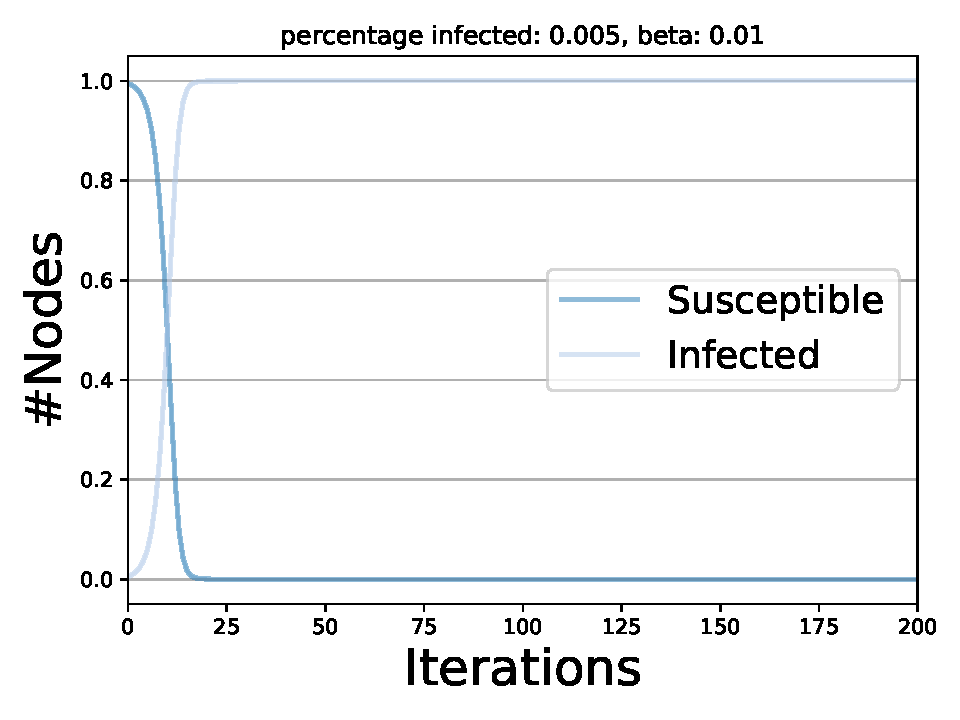
\includegraphics{images/spreading/si/diffusion_er.pdf}
            }
            \caption{}
            \label{diff_si_er}
        \end{subfigure}
        \begin{subfigure}{0.45\textwidth}
            \resizebox{\textwidth}{!}{
                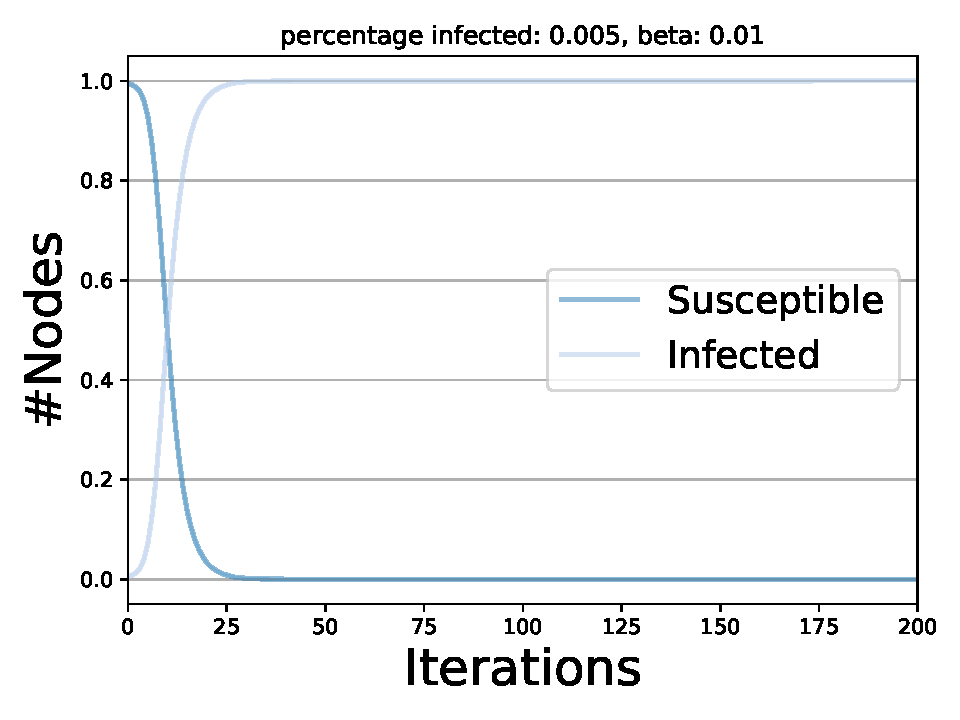
\includegraphics{images/spreading/si/diffusion_ba.pdf}
            }
            \caption{}
            \label{diff_si_ba}
        \end{subfigure}
        \begin{subfigure}{0.45\textwidth}
            \resizebox{\textwidth}{!}{
                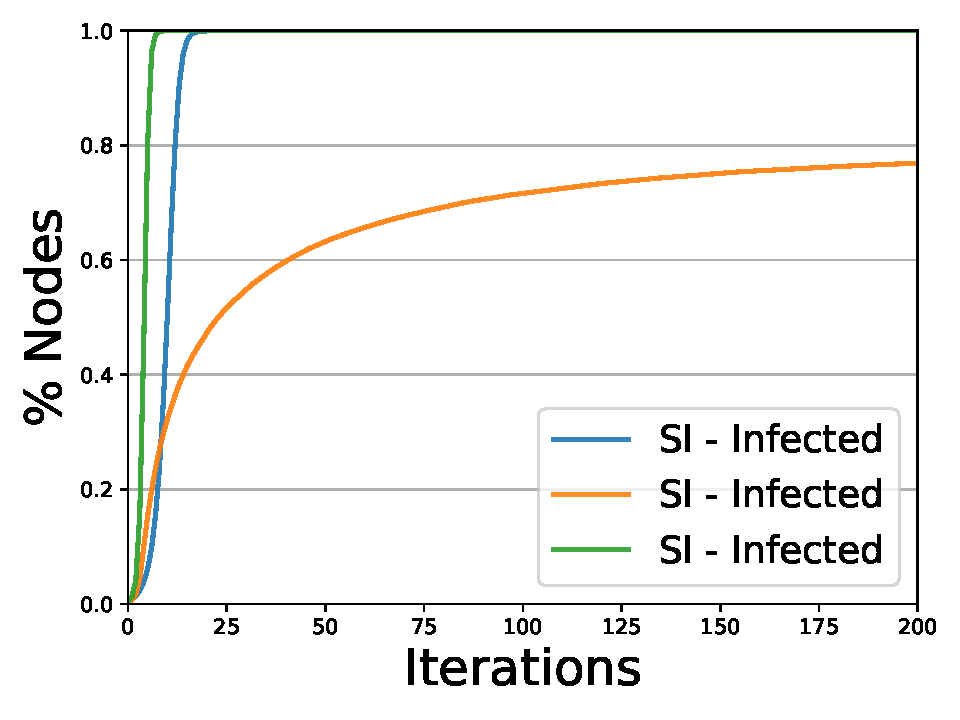
\includegraphics{images/spreading/si/trend_comparison.pdf}
            }
            \caption{}
            \label{diff_si_comparison}
        \end{subfigure}
        \caption{In Figure \ref{diff_si} we can see the diffusion graph for the original network, while in Figure
        \ref{diff_si_er} and in Figure \ref{diff_si_ba} we can see the diffusion graph for the Erdős–Rényi and
        Barabási–Albert networks, respectively. In Figure \ref{diff_si_comparison} we can see a comparison between
        the infection rate of the three networks.}
        \label{diff_si_total}
    \end{figure}
    For the \textbf{Susceptible-Infected} model we've started with a $0.005\%$ of the total population ($3$ nodes)
    of each network being infected, and we've choosed a value of $0.01$ for the infection rate $\beta$. As you can
    see from Figure \ref{diff_si_total}, the original network is the only one that doesn't reach the saturation
    regime, while the other networks reach it within the first $25$ iterations of the model. This is due to the fact
    that both the Erdős–Rényi and the Barabási–Albert network are extremely connected, hence it is more easy for the
    infection to spread among the nodes.

% section si_model (end)

\section{SIS model} % (fold)
\label{sec:sis_model}
    \begin{figure}[H]
        \centering
        \begin{subfigure}{0.45\textwidth}
            \resizebox{\textwidth}{!}{
                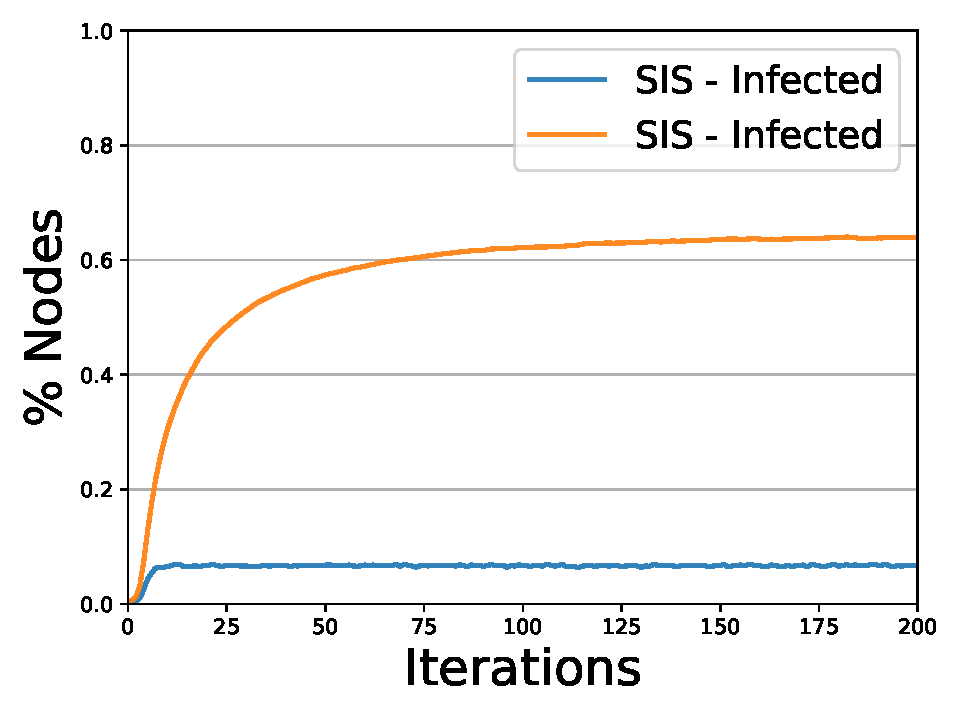
\includegraphics{images/spreading/sis/diffusion_original_comparison.pdf}
            }
            \caption{}
            \label{diff_sis}
        \end{subfigure}
        \begin{subfigure}{0.45\textwidth}
            \resizebox{\textwidth}{!}{
                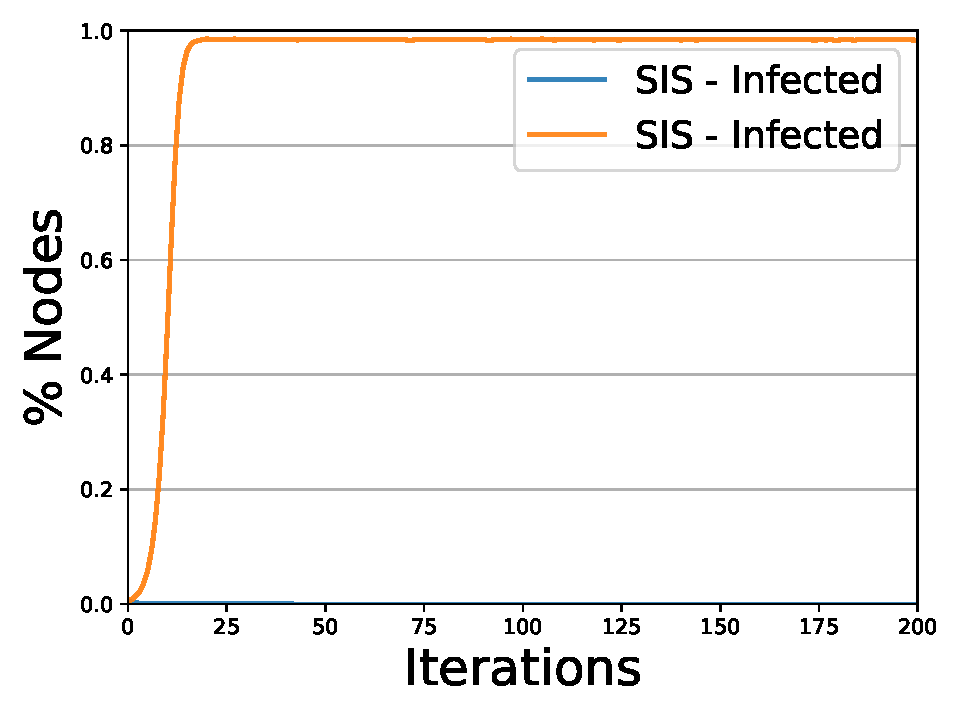
\includegraphics{images/spreading/sis/diffusion_er_comparison.pdf}
            }
            \caption{}
            \label{diff_sis_er}
        \end{subfigure}
        \begin{subfigure}{0.45\textwidth}
            \resizebox{\textwidth}{!}{
                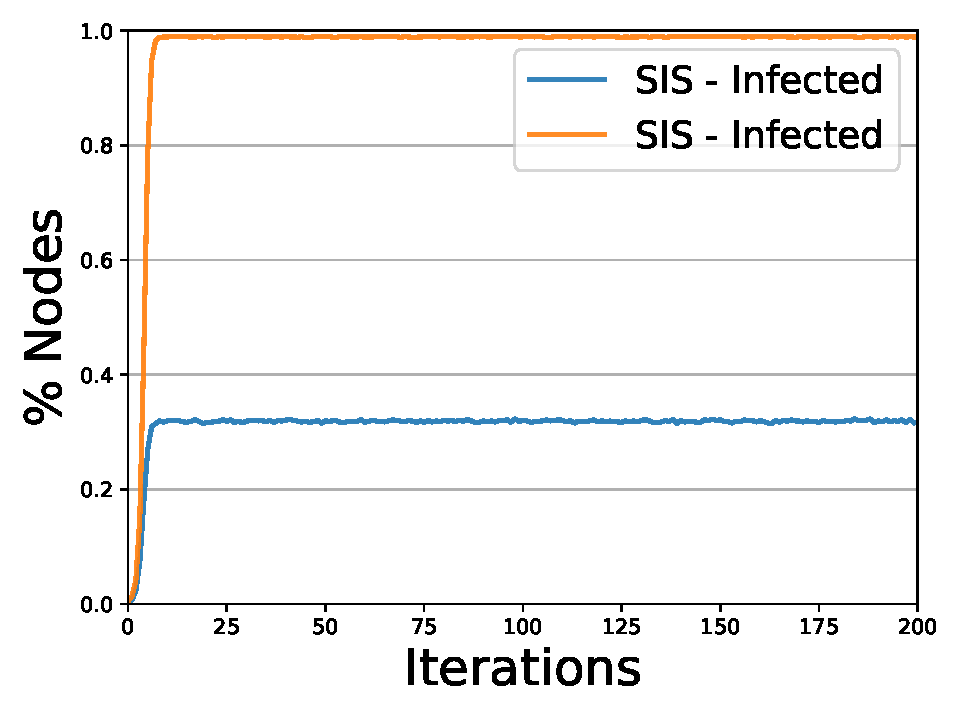
\includegraphics{images/spreading/sis/diffusion_ba_comparison.pdf}
            }
            \caption{}
            \label{diff_sis_ba}
        \end{subfigure}
        \caption{In Figure \ref{diff_sis} we can see the comparison between the endemic state, in orange, and the
        disease free state, in blue, for the original network. The same comparison can be observed for the
        Erdős–Rényi and the Barabási–Albert network, respectively, in Figure \ref{diff_sis_er} and
        \ref{diff_sis_ba}}
        \label{diff_sis_total}
    \end{figure}
    For the \textbf{Susceptible-Infected-Susceptible} model, thanks to the introduction of the recovery rate $\mu$,
    we can model two possible outcomes for the epidemic: the \textbf{endemic state}, characterized by a low recovery
    rate and by the fraction of infected individuals that follows a logistic curve similar to the one observed for
    the SI model, for which $\mu < \beta\langle k \rangle$, and the \textbf{disease free} state, characterized by a
    sufficiently high recovery rate, for which $\mu > \beta\langle k \rangle$. A comparison between this two states
    is represented for every network in Figure \ref{diff_sis_total}.

% section sis_model (end)

\section{SIR model} % (fold){}
\label{sec:sir_model}
    The key characteristic of the \textbf{Susceptible-Infected-Recovered} model consist in introducing the
    probability $\gamma$ for the individuals to recover from the disease and hence to be "removed" from the
    population instead of returning to the susceptible state. We have choosen to test this model either for the case
    in which $\gamma$ is smaller than $\beta$ and the other way around. The graphs representing this different
    situations for all the three networks are visible in Figure \ref{diff_sir_total}.
    \begin{figure}
        \begin{subfigure}{0.33\textwidth}
            \resizebox{\textwidth}{!}{
                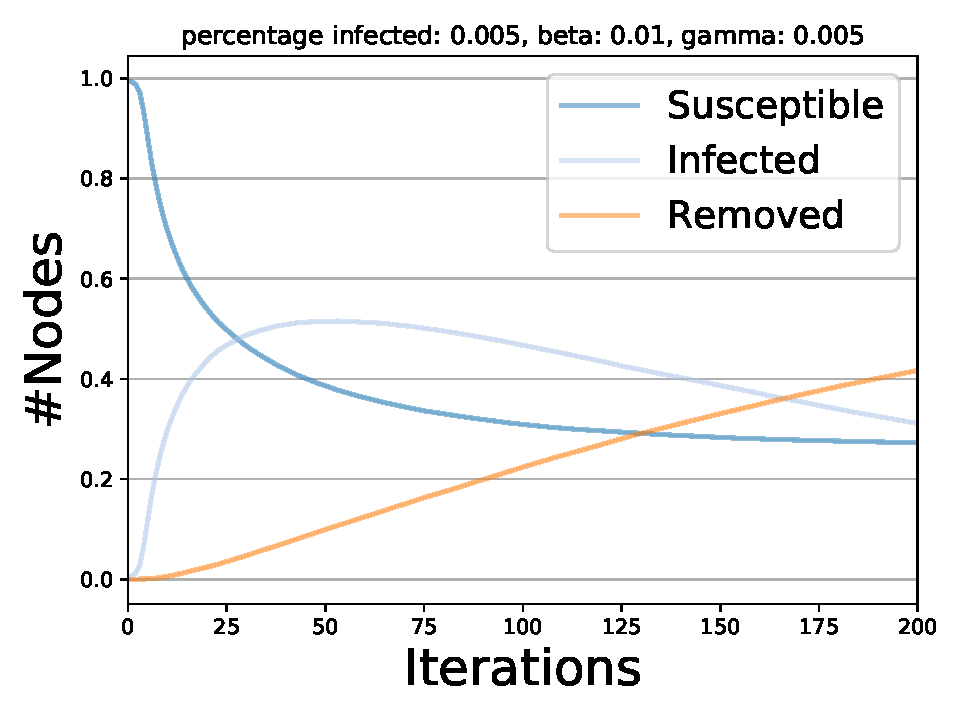
\includegraphics{images/spreading/sir/diffusion_smaller.pdf}
            }
            \caption{}
            \label{diff_sir_smaller}
        \end{subfigure}
        \begin{subfigure}{0.33\textwidth}
            \resizebox{\textwidth}{!}{
                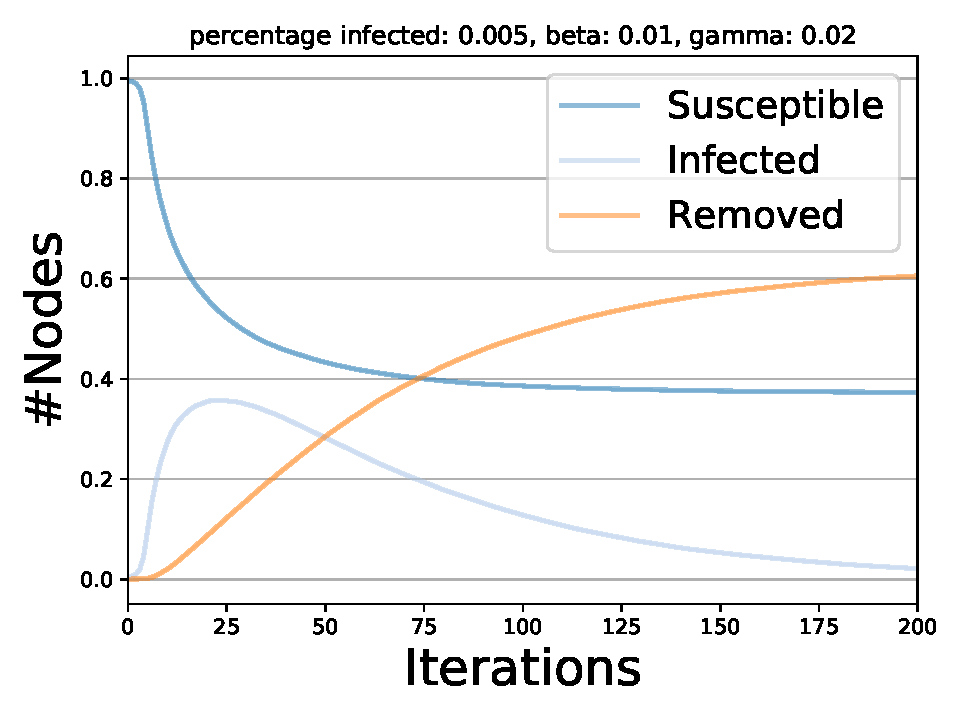
\includegraphics{images/spreading/sir/diffusion_greater.pdf}
            }
            \caption{}
            \label{diff_sir_greater}
        \end{subfigure}
        \begin{subfigure}{0.33\textwidth}
            \resizebox{\textwidth}{!}{
                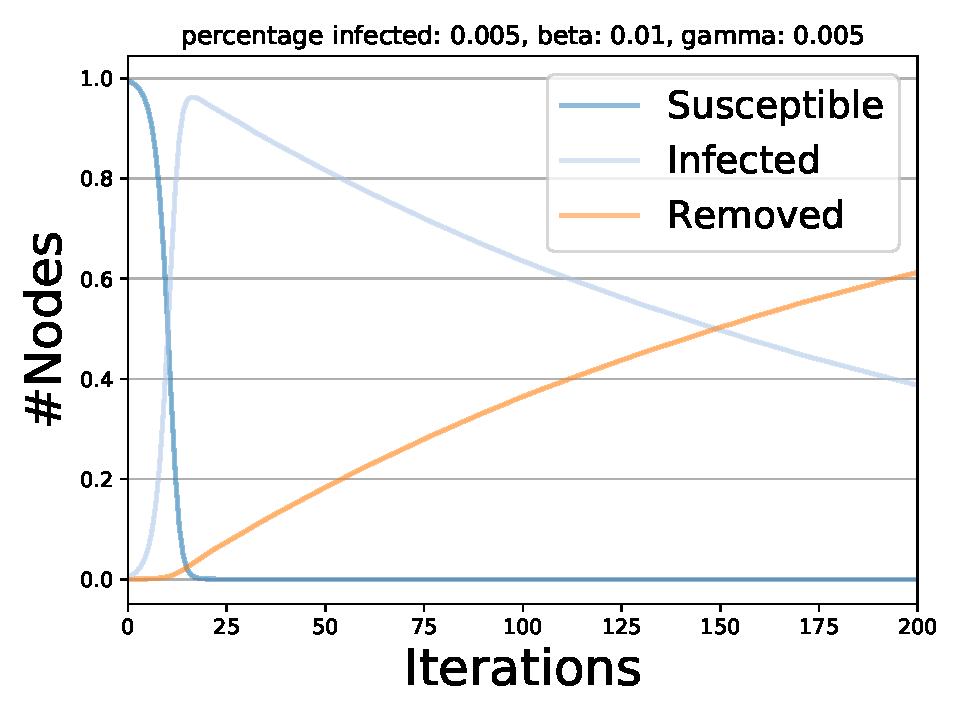
\includegraphics{images/spreading/sir/diffusion_er_smaller.pdf}
            }
            \caption{}
            \label{diff_sir_er_smaller}
        \end{subfigure}
        \begin{subfigure}{0.33\textwidth}
            \resizebox{\textwidth}{!}{
                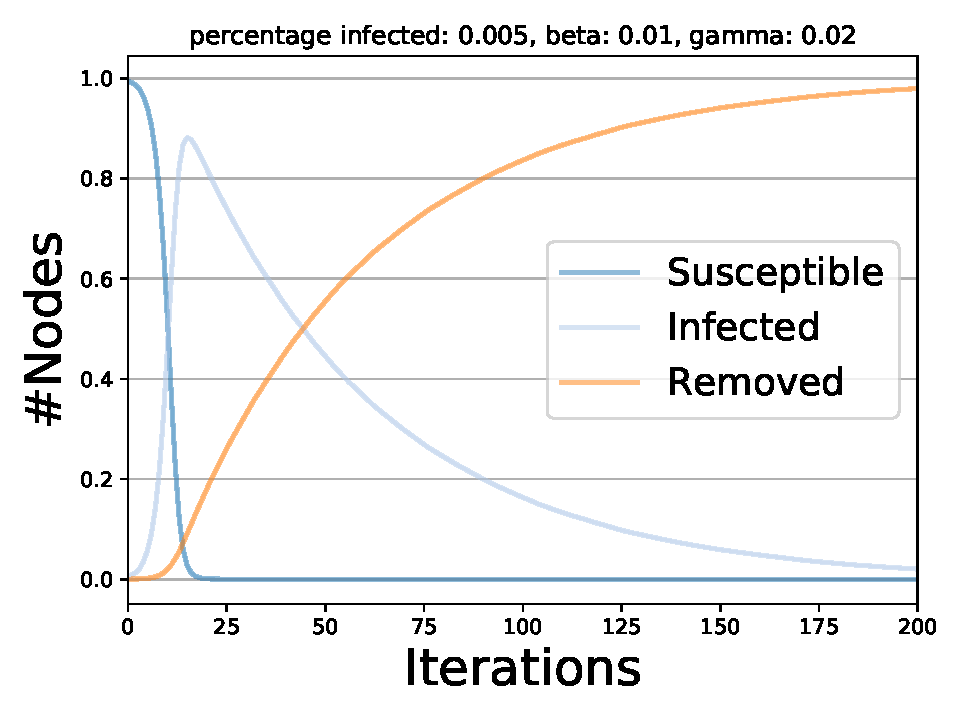
\includegraphics{images/spreading/sir/diffusion_er_greater.pdf}
            }
            \caption{}
            \label{diff_sir_er_greater}
        \end{subfigure}
        \begin{subfigure}{0.33\textwidth}
            \resizebox{\textwidth}{!}{
                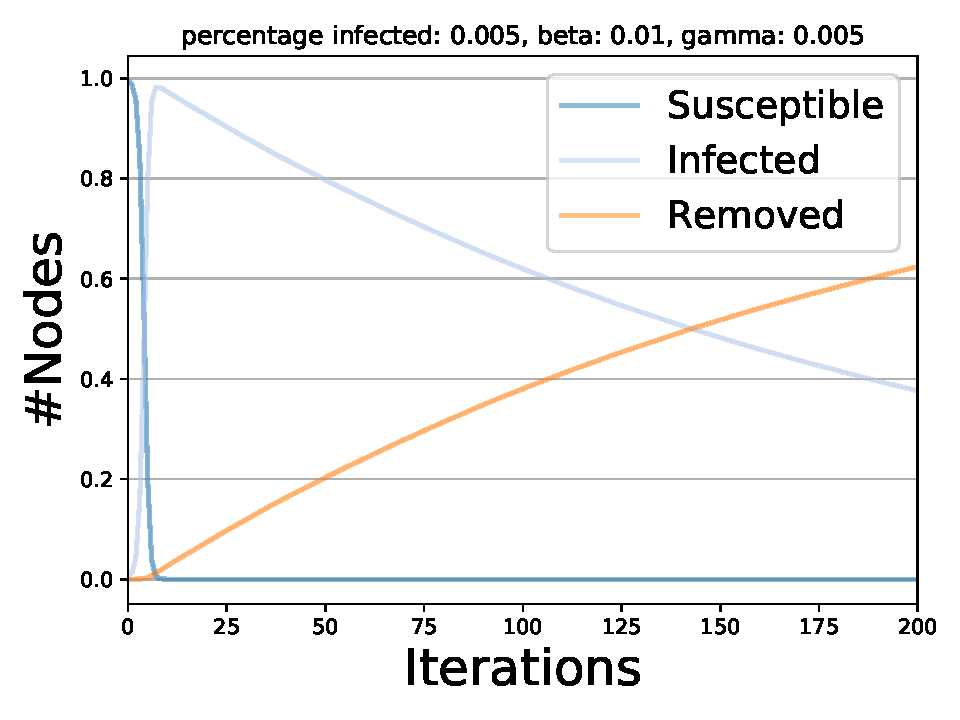
\includegraphics{images/spreading/sir/diffusion_ba_smaller.pdf}
            }
            \caption{}
            \label{diff_sir_ba_smaller}
        \end{subfigure}
        \begin{subfigure}{0.33\textwidth}
            \resizebox{\textwidth}{!}{
                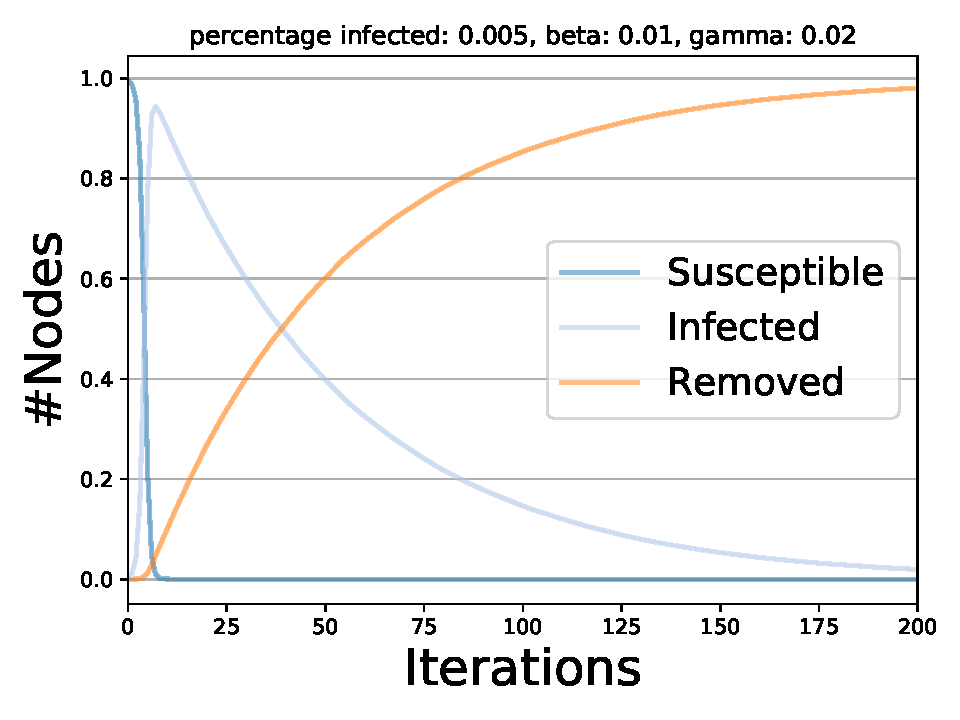
\includegraphics{images/spreading/sir/diffusion_ba_greater.pdf}
            }
            \caption{}
            \label{diff_sir_ba_greater}
        \end{subfigure}
        \caption{In Figure \ref{diff_sir_smaller} and \ref{diff_sir_greater} we can see the representation of the
        diffusion on the original network both for the case in which $\gamma$ is smaller than $\beta$ and the other
        way around. The same kind of representation is plotted for the Erdős–Rényi network in Figure
        \ref{diff_sir_er_smaller} and \ref{diff_sir_er_greater} and for the Barabási–Albert network in Figure
        \ref{diff_sir_ba_smaller} and \ref{diff_sir_ba_greater}.}
        \label{diff_sir_total}
    \end{figure}

% section sir_model (end)

\section{Threshold model} % (fold)
\label{sec:threshold_model}
    Finally we describe the application of the \textbf{Threshold model} both on the original network and the
    synthetic ones. In order to test this model we've choosen to apply a threshold $\tau$ eguals to $0.10$, the
    diffusion of the infection for this model is represented in Figure \ref{diff_thr_total}. As we can see, for the
    original network we have that almost all the nodes become infected within the first $20$ model's iterations,
    due to the fact that the value choosen for the threshold results to be sufficient for the spreading of the
    infection. If we change the threshold's value, this time using $0.20$, we can observe that the
    original network become immune to the infection, thanks to its internal structure. We can observe
    the same immunity in the Erdős–Rényi and Barabási–Albert network for the original threshold's value.
    \begin{figure}[H]
        \centering
        \begin{subfigure}{0.33\textwidth}
            \resizebox{\textwidth}{!}{
                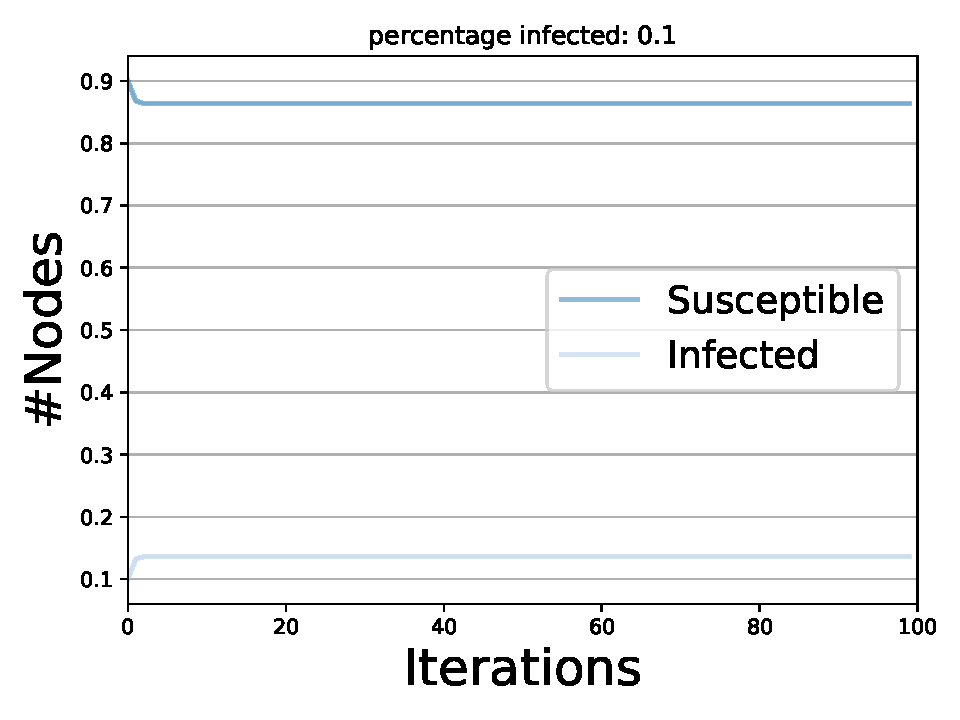
\includegraphics{images/spreading/threshold/diffusion.pdf}
            }
            \caption{}
            \label{diff_thr}
        \end{subfigure}
        \begin{subfigure}{0.33\textwidth}
            \resizebox{\textwidth}{!}{
                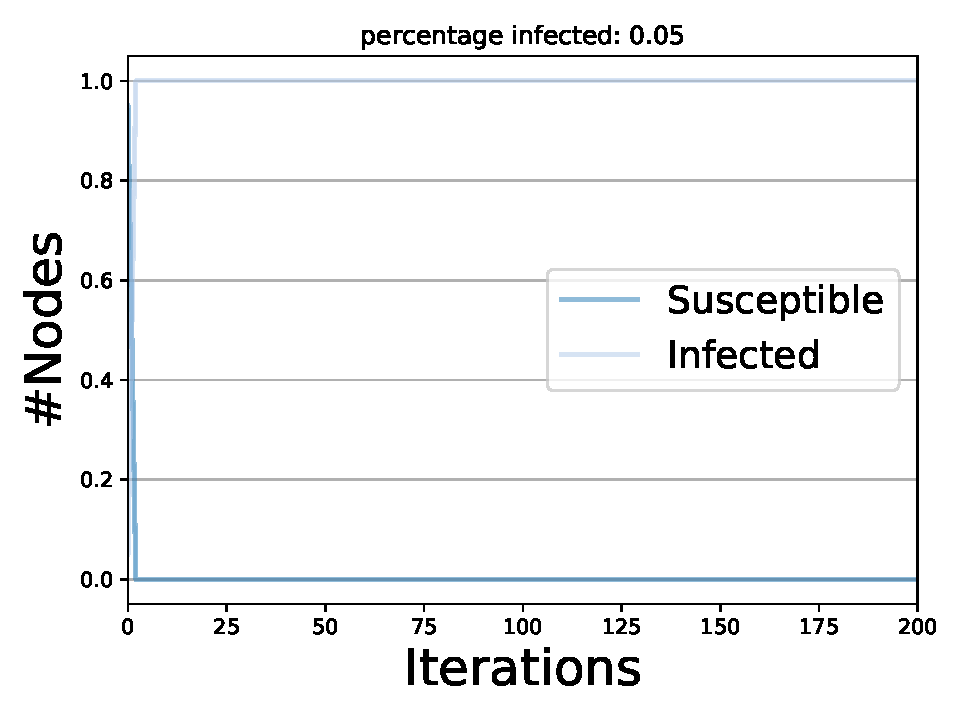
\includegraphics{images/spreading/threshold/diffusion_er.pdf}
            }
            \caption{}
            \label{diff_thr_er}
        \end{subfigure}
        \begin{subfigure}{0.33\textwidth}
            \resizebox{\textwidth}{!}{
                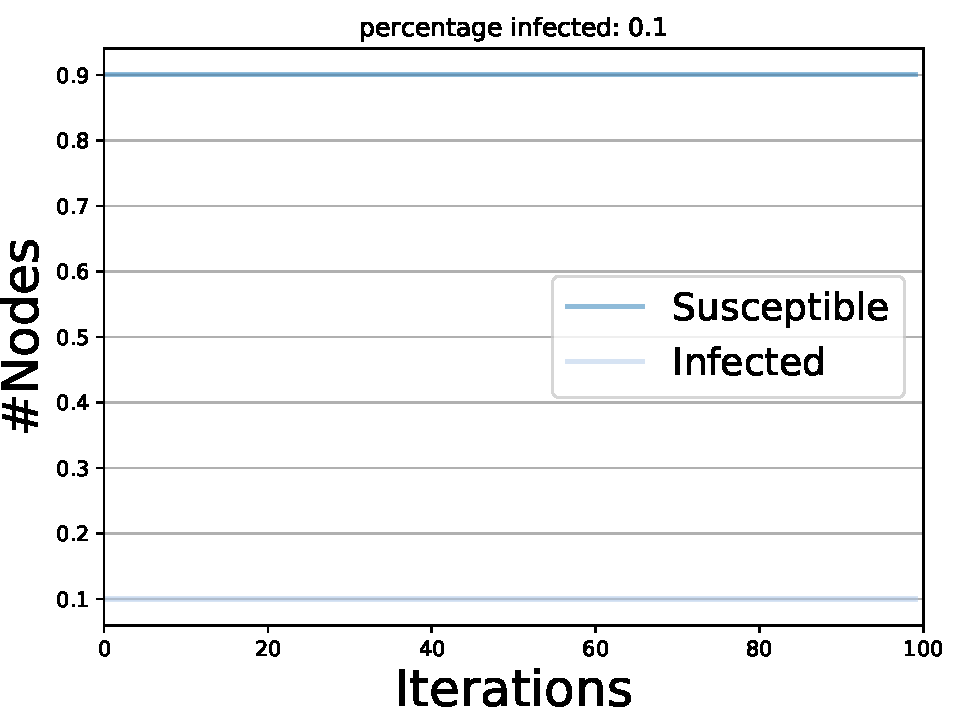
\includegraphics{images/spreading/threshold/diffusion_ba.pdf}
            }
            \caption{}
            \label{diff_thr_ba}
        \end{subfigure}
        \begin{subfigure}{0.33\textwidth}
            \resizebox{\textwidth}{!}{
                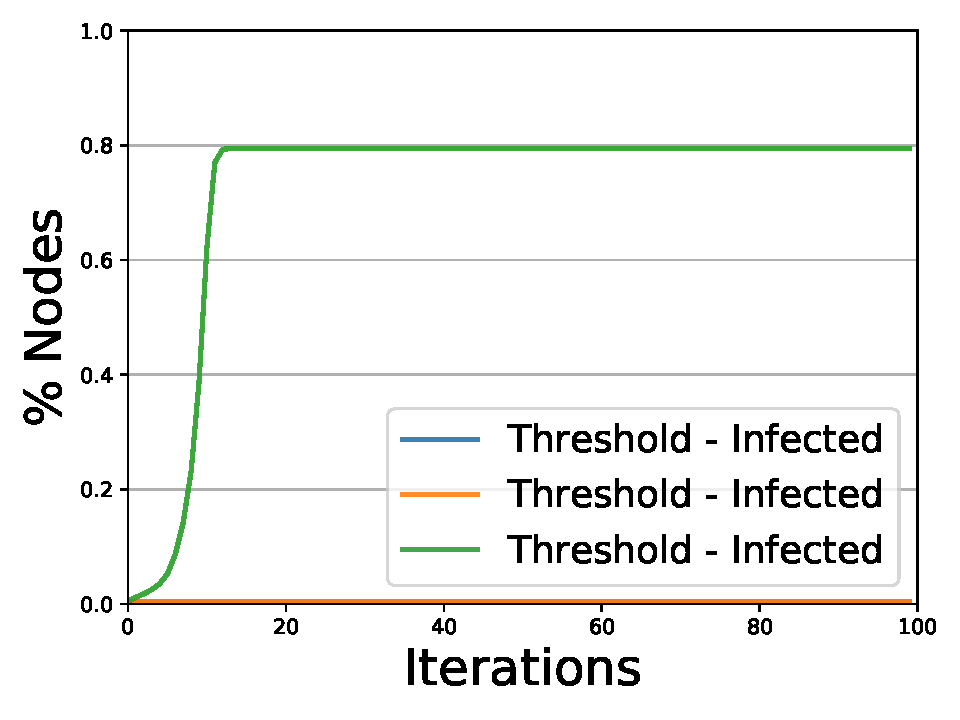
\includegraphics{images/spreading/threshold/trend_comparison.pdf}
            }
            \caption{}
            \label{diff_thr_comparison}
        \end{subfigure}
        \caption{In Figure \ref{diff_thr} is represented the diffusion of the infection for the original network,
        while in Figure \ref{diff_thr_er} and \ref{diff_thr_ba} are represented the cases for the Erdős–Rényi and
        the Barabási–Albert network, respectively. A comparison between the three networks is represented in Figure
        \ref{diff_thr_comparison}.}
        \label{diff_thr_total}
    \end{figure}

% section threshold_model (end)

% chapter spreading (end)


    \chapter{Summary}


\printbibliography[title={References}]


\end{document}
